\chapter{Model formulations}

The model solves coupled 2D horizontal equations for wave propagation, flow, sediment transport and bottom changes, for varying (spectral) wave and flow boundary conditions. Because the model takes into account the variation in wave height in time (long known to surfers) it resolves the long wave motions created by this variation. This so-called `surf beat' is responsible for most of the swash waves that actually hit the dune front or overtop it. With this innovation the XBeach model is better able to model the development of the dune erosion profile, to predict when a dune or barrier island will start overwashing and breaching and to model the developments throughout these phases.

\section{ Coordinate system}

XBeach uses a coordinate system where the computational x-axis is always oriented towards the coast, approximately perpendicular to the coastline, and the y-axis is alongshore, see Figure 2.1 . This coordinate system is defined relative to world coordinates $(x_{w},y_{w})$ through the origin $(x_{ori},y_{ori})$ and the orientation alfa, defined counter-clockwise w.r.t. the $x_{w}$-axis (East). The grid size in x- and y-direction may be variable but the grid must be rectilinear.

\begin{figure}[h]
  \centering
  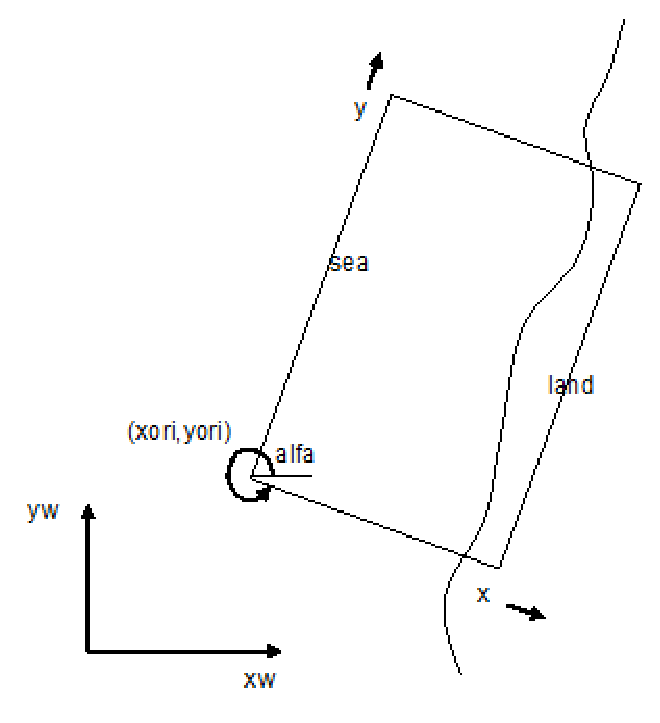
\includegraphics[width=0.6\textwidth]{image1}
  \caption{Coordinate system}
  \label{fig:image1}
\end{figure}

\section{ Grid Setup}

The grid applied is a staggered grid, where the bed levels, water levels, water depths and concentrations are defined in cell centers, and velocities and sediment transports are defined in u- and v-points, viz. at the cell interfaces. In the wave energy balance, the energy, roller energy and radiation stress are defined at the cell centers, whereas the radiation stress gradients are defined at u- and v-points, see Figure 2.2.

Velocities at the u- and v-points are denoted by uu and vv respectively; velocities u and v at the cell centers are obtained by interpolation and are for output purpose only. The water level, zs, and the bed level, zb, are both defined positive upward. uv and vu are the u-velocity at the v-grid point and the v-velocity at the u-grid point respectively. These are obtained by interpolation of the values of the velocities at the four surrounding grid points. 

The model solves coupled 2D horizontal equations for wave propagation, flow, sediment transport and bottom changes, for varying (spectral) wave and flow boundary conditions. Because the model takes into account the variation in wave height in time (long known to surfers) it resolves the long wave motions created by this variation. This so-called `surf beat' is responsible for most of the swash waves that actually hit the dune front or overtop it. With this innovation the XBeach model is better able to model the development of the dune erosion profile, to predict when a dune or barrier island will start overwashing and breaching and to model the developments throughout these phases.

\section{ Wave action equation solver}

The wave forcing in the shallow water momentum equation is obtained from a time dependent version of the wave action balance equation. Similar to Delft University's (stationary) HISWA model \citep{Holthuijsen1989}, the directional distribution of the action density is taken into account whereas the frequency spectrum is represented by a frequency, best represented by the spectral parameter $f_{m,-1.0}$. The wave action balance is then given by:

\begin{equation} \label{ZEqnNum711560} 
\frac{\partial A}{\partial t} +\frac{\partial c_{x} A}{\partial x} +\frac{\partial c_{y} A}{\partial y} +\frac{\partial c_{\theta } A}{\partial \theta } =-\frac{D_{w} }{\sigma }  
\end{equation} 

with the wave action:

\begin{equation} \label{2.2)} 
A(x,y,t,\theta )=\frac{S_{w} (x,y,t,\theta )}{\sigma (x,y,t)}  
\end{equation} 

where $\theta $ represents the angle of incidence with respect to the x-axis, $S_{w}$ represents the wave energy density in each directional bin and $\sigma$ the intrinsic wave frequency. The wave action propagation speeds in x- and y-direction are given by:

\begin{equation} \label{2.3)} 
\begin{array}{l} {c_{x} (x,y,t,\theta )=c_{g} \cos (\theta )+u^{L} } \\ {c_{y} (x,y,t,\theta )=c_{g} \sin (\theta )+v^{L} } \end{array} 
\end{equation} 

With \textit{u${}^{L}$} and \textit{v${}^{L}$} the cross-shore and alongshore depth-averaged Lagrangian velocities respectively (defined below), and the group velocity \textit{c${}_{g}$} obtained from linear theory. If wave-current interaction is turned off (\textit{wci=0}) then the last term in either equation is not taken into account.

The propagation speed in $\theta $-space is obtained from:

\begin{equation} \label{ZEqnNum944441} 
\begin{array}{l} {c_{\theta } (x,y,t,\theta )=\frac{\sigma }{\sinh 2kh} \left(\frac{\partial h}{\partial x} \sin \theta -\frac{\partial h}{\partial y} \cos \theta \right)+\cos \theta \left(\sin \theta \frac{\partial u}{\partial x} -\cos \theta \frac{\partial u}{\partial y} \right)+} \\ {\, \, \, \, \, \, \, \, \, \, \, \, \, \, \, \, \, \, \, \, \, \, \, \, \, \, \, \, \, \, \, \, \, \, \, \, \, \, \, \, \, \, \, \, \, \, \, \, \, \, \, \, \, \, \, \, \, \, \, \, \, \, \, \, \, \, \, \, \, \, \, \, \, \, \, \, \, \, \, \, \, \, \, \, \, \, \, \, \, \, \, \, \, +\sin \theta \left(\sin \theta \frac{\partial v}{\partial x} -\cos \theta \frac{\partial v}{\partial y} \right)} \end{array} 
\end{equation} 

taking into account bottom refraction (first term on the RHS) and current refraction (last two terms on the RHS) and \textit{h} is the total water depth. If wave-current interaction is turned off (\textit{wci=0}) then the last two terms are not taken into account.

The wave number \textit{k} is obtained from the eikonal equations:

\begin{equation} \label{2.5)} 
\begin{array}{l} {\frac{\partial k_{x} }{\partial t} +\frac{\partial \omega }{\partial x} =0} \\ {\frac{\partial k_{y} }{\partial t} +\frac{\partial \omega }{\partial y} =0} \end{array} 
\end{equation} 

where the subscripts refer to the direction of the wave vector components and $\omega $ represents the absolute radial frequency. The wave number is then obtained from:

\begin{equation} \label{2.6)} 
k=\sqrt{k_{x}^{2} +k_{y}^{2} }  
\end{equation} 

The absolute radial frequency is given by:

\begin{equation} \label{2.7)} 
\omega =\sigma +k_{x} u^{L} +k_{y} v^{L}  
\end{equation} 

and the intrinsic frequency is obtained from the linear dispersion relation. If wave-current interaction is turned off (\textit{wci=0}) then the last two terms are not taken into account.

The total wave energy dissipation, i.e. directionally integrated, due to wave breaking is modelled according to \citet{Roelvink1993a}, which is coded as \textit{break=1}:

\begin{equation} \label{2.8)} 
\begin{array}{l} {\bar{D}_{w} =2\frac{\alpha }{T_{rep} } Q_{b} E_{w} } \\ {Q_{b} {\rm =1-exp}\left({\rm -}\left(\frac{{\rm H}_{{\rm rms}} }{H_{\max } } \right)^{n} \right),\, \, \, \, H=\sqrt{\frac{8E_{w} }{\rho g} } ,\quad H_{\max } =\frac{\gamma \tanh kh}{k} } \end{array} 
\end{equation} 

with $\alpha =O\eqref{GrindEQ__1_}$, \textit{r} the water density, $\gamma $ the breaker index (a free parameter) and the total wave energy is given by:

\begin{equation} \label{2.9)} 
E_{w} (x,y,t)=\int _{0}^{2\pi }S_{w} (x,y,t,\theta )d\theta  .  
\end{equation} 

In a variation of the above, one could also state (\textit{break = 3)}

\begin{equation} \label{2.10)} 
\bar{D}_{w} =2\frac{\alpha }{T_{rep} } Q_{b} E_{w} \frac{H_{rms} }{h}  
\end{equation} 

Finally, Roelvink and Daly (\textit{break = }4) developed a breaking formulation based on \eqref{GrindEQ__2_10_} where the fraction of breaking waves is modelled as

\begin{equation} \label{2.11)} 
\left\{\begin{array}{l} {Q_{b} =1\quad if\quad H_{rms} >\gamma h} \\ {Q_{b} =0\quad if\quad H_{rms} <\gamma _{2} h} \end{array}\right.  
\end{equation} 

which states that waves are fully breaking is the wave height exceeds a threshold and stop breaking if the wave height fall below another threshold. Details are in \citet{DalyRoelvink2010}.

In the stationary case, we apply \citet{Baldock1998} (\textit{break = 2) } which states 
\begin{equation} \label{2.12)} 
\bar{D}=\frac{1}{4} \alpha Q_{b} \rho gf_{rep} \left(H_{b}^{2} +H_{rms}^{2} \right) 
\end{equation} 

With $\alpha = O(1)$ and $f_rep$ representing a representative intrinsic frequency. The fraction of breaking waves is given by:

\begin{equation} \label{2.13)} 
Q_{b} =\exp \left[-\left(\frac{H_{b}^{2} }{H_{rms}^{2} } \right)\right] 
\end{equation} 

Where the breaking wave height is:

\begin{equation} \label{2.14)} 
H_{b} =\frac{0.88}{k} \tanh \left[\frac{\gamma kh}{0.88} \right] 
\end{equation} 

And $\gamma$ is a calibration parameter. 

In either instationary or stationary case the total wave dissipation, $\bar{D}$, is distributed proportionally over the wave directions:

\begin{equation} \label{2.15)} 
D_{w} (x,y,t,\theta )=\frac{S_{w} (x,y,t,\theta )}{E_{w} (x,y,t)} \bar{D}_{w} (x,y,t) 
\end{equation} 

The bed friction dissipation is modelled as

\begin{equation} \label{2.16)} 
D_{f} =\frac{2}{3} \rho \pi f_{w} \left(\frac{\pi H}{T_{rep} \sinh kh} \right)^{3}  
\end{equation} 

This closes the set of equations for the wave action balance. Given the spatial distribution of the wave action and therefore wave energy the radiation stresses can be evaluated (using linear wave theory):

\begin{equation} \label{ZEqnNum727357} 
\begin{array}{l} {S_{xx,w} (x,y,t)=\int \left(\frac{c_{g} }{c} \left(1+\cos ^{2} \theta \right)-\frac{1}{2} \right)S_{w} d\theta  } \\ {S_{xy,w} (x,y,t)=S_{yx,w} =\int \sin \theta \cos \theta \left(\frac{c_{g} }{c} S_{w} \right) d\theta } \\ {S_{yy,w} (x,y,t)=\int \left(\frac{c_{g} }{c} \left(1+\sin ^{2} \theta \right)-\frac{1}{2} \right)S_{w} d\theta  } \end{array} 
\end{equation} 

\paragraph{Instationary vs. stationary wave solver}

For situations where infragravity motions play an important role the wave and roller equations must be solved in instationary, wave-group resolving mode (\textit{instat=1, by default)}. For some applications which do not focus on swash motions and where surfbeats are small, we have implemented an option (\textit{instat=0}) to solve the stationary problem directly using a forward marching technique, where the equations are solved grid row by grid row in an iterative fashion. The wave module is then called every \textit{wavint} seconds rather than each time step, which often means a large reduction in computation time. 

\subsection{ Wave boundary conditions}
\paragraph{Offshore wave boundary conditions}

At present, a number of wave boundary conditions can be specified at the offshore boundary. These are numbered ``instat=0'' through ``instat=41''. The overview is as follows:

\begin{tabular}{|p{0.5in}|p{0.8in}|p{2.6in}|} \hline 
instat & abbreviated name & description \\ \hline 
0 & stat & stationary wave boundary condition (sea state) \\ \hline 
1 & bichrom & bichromatic (two wave component) waves \\ \hline 
2 & ts\_1 & first-order timeseries of waves (generated outside XBeach) \\ \hline 
3 & ts\_2 & second-order timeseries of waves (generated outside XBeach) \\ \hline 
4 & jons & wave groups generated using a parametric (Jonswap) spectrum \\ \hline 
5 & swan & wave groups generated using a SWAN 2D output file \\ \hline 
6 & vardens & wave groups generated using a formatted file \\ \hline 
7 & reuse & reuse of wave conditions \\ \hline 
8 & nonh & boundary conditions for nonhydrostatic option \\ \hline 
9 & off & no wave boundary condition \\ \hline 
40 & stat\_table & a sequence of stationary conditions (sea states) \\ \hline 
41 & jons\_table & a sequence of time-varying wave groups \\ \hline 
\end{tabular}

In the params.txt file the boundary conditions options can be invoked using either the number (``instat=3'' for instance) or by using the name ``instat=ts\_2''. The name must be lower case and match exactly.

\underbar{Stationary wave boundary conditions (}\textit{\underbar{instat =}}\underbar{ 0).} 

In this case a uniform, constant wave energy distribution is set, based on given values of H${}_{rms}$, T${}_{m01}$, direction and power of directional distribution function.

\begin{equation} \label{2.18)} 
\begin{array}{l} {e_{0} (\vartheta )=E_{mean} \frac{\cos ^{m} \left(\vartheta -\vartheta _{m} \right)}{\sum _{\vartheta _{\min } }^{\vartheta _{\max } }\cos ^{m} \left(\vartheta -\vartheta _{m} \right)\Delta \vartheta  } \, \, \, \, \, \, ,\, \, \left|\vartheta -\vartheta _{m} \right|<\pi /2} \\ {\, \, \, \, \, \, \, \, \, \, \, \, \, \, \, \, \, E_{mean} =\frac{1}{8} \rho gH_{rms}^{2} } \end{array} 
\end{equation} 

\underbar{Wave energy varying periodically in time (}\textit{\underbar{instat =}}\underbar{ 1):}

In this case regular wave groups (i.e. bichromatic waves) are specified.

\begin{equation} \label{2.19)} 
\begin{array}{l} {e_{0} (\vartheta )=E_{mean} \frac{\cos ^{m} \left(\vartheta -\vartheta _{m} \right)}{\sum _{\vartheta _{\min } }^{\vartheta _{\max } }\cos ^{m} \left(\vartheta -\vartheta _{m} \right)\Delta \vartheta  } *\frac{1}{2} \left(1\, +\, \cos \left(2\pi \left(\frac{t}{T_{long} } -\frac{y}{L_{long} } \right)\right)\right),} \\ {\, \, \, \, \, \, \, \, \, \, \, \, \, \, \, \, \, L_{long} =\frac{c_{g} T_{long} }{\sin (\vartheta _{m} )} } \end{array} 
\end{equation} 

\underbar{First-order longcrested, irregular wave groups (}\textit{\underbar{instat =}}\underbar{ 2)}

In this case E is read in as a function of time; the timeseries is shifted along the y-axis to account for the oblique incidence.

\begin{equation} \label{2.20)} 
\begin{array}{l} {e_{0} (\vartheta ,y)=E_{t-\tau (y)} \frac{\cos ^{m} \left(\vartheta -\vartheta _{m} \right)}{\sum _{\vartheta _{\min } }^{\vartheta _{\max } }\cos ^{m} \left(\vartheta -\vartheta _{m} \right)\Delta \vartheta  } ,} \\ {\, \, \, \, \, \, \, \, \, \, \, \, \, \, \, \, \, \tau (y)=\frac{y\, \sin (\vartheta _{m} )}{c_{g} } } \end{array} 
\end{equation} 

This time series needs to be made by a separate routine (not part of XBeach). An example of the required input format is given in the Appendix B

Second-order longcrested, irregular wave groups (\textit{instat =} 3)

In this case a bound wave is added to the wave groups using \citet{LonguetHigginsStewart1964} theory. The format is prescribed in Appendix B

\underbar{Standard JONSWAP} \underbar{spectrum, based on user-input spectrum coefficients (}\textit{\underbar{instat =}}\underbar{ 4)}

With this option alongshore varying timeseries of the wave energy E and bound long wave z${}_{s}$ are generated on the basis of a specified analytical 2D Jonswap-type spectrum. With this option realistic second-order bound, directionally-spread seas can be created. 

The spectrum is determined by the peak period, wave height, spectral peakedness, mean angle and directional spreading (see section 5.7 for details on the input values). The routine follows the procedure as outlined by \citet{VanDongeren2003}, see next paragraph.

\underbar{Unmodified SWAN 2D spectrum output file (}\textit{\underbar{instat =}}\underbar{ 5)}

\underbar{}

This option uses a SWAN 2D output file (sp2 file) in unmodified form. The procedure to calculate the boundary conditions is analoguous to the instat=4 option.

\underbar{Formatted variance-density spectrum file (}\textit{\underbar{instat =}}\underbar{ 6)}

\underbar{}

This option uses a formatted variance-density spectrum file, which needs to adhere to certain criteria (see section 5.5). On the basis of this formatted spectrum, boundary conditions are calculated using the procedure as outlined under \textit{instat =} 4.

\underbar{Reuse boundary condition files from an earlier XBeach simulation (}\textit{\underbar{instat =}}\underbar{ 7)}

\underbar{}

If the user does not wish to recalculate spectrum-based boundary condition files or specifically wants to reuse the spectrum-based boundary condition files of another XBeach simulation, it is possible to do so. In this case the user should select `\textit{instat =} 7' in params.txt. No further wave boundary condition data need be given in params.txt. Obviously, the calculation grid should remain the same between runs, as the angles and number of grid points are embedded in the boundary condition files. In order to use instat 7, the user should copy \textit{ebcflist.bcf} and \textit{qbcflist.bcf} to the current directory. Additionally, the user should also copy all files listed in \textit{ebcflist.bcf} and \textit{qbcflist.bcf}. Generally, these files have E\_ and q\_ prefixes.

With instat=4, 5 and 6 time-varying (on the scale of wave groups) boundary conditions are computed on the basis of stationary input spectra. It is also possible to use a sequence of varying spectra to compute boundary conditions which not only vary on the time scale of the wave groups but also have a variation on the longer timescale. The procedure is similar to the one described above, only the implementation is through the specification of a list of spectrum files, see section 5.7.

B\underbar{oundary conditions for non-hydrostatic model (}\textit{\underbar{instat =}}\underbar{ 8)}

\underbar{}

XBeach can be ran as a non-hydrostatic model, which is essentially the nonlinear shallow water  equations with dispersion terms and without a wave-action driver. The boundary conditions are described in a separate chapter and are activated using instat=8

No boundary condition \underbar{(}\textit{\underbar{instat =}}\underbar{ 9)}

\underbar{}

This is a simple ``no wave action'' boundary condition. It still allows for a tidal record to be specified, however through the zs0file parameter.

Sequence of stationary sea states (\textit{instat = 40})\underbar{}

\underbar{}

While instat=0 specifies one stationary sea state (stationary in the sense that there are no wave groups), it is also possible to specify a series of seastates, each with a duration. This is done through a file as

instat   = 40

bcfile   = jonswap1.txt

where the name of the bcfile is free, but the structure of the contents is not. It should contain lines with

Hm0, Tp, angle, gamma \eqref{GrindEQ__3_3_}, spreading, duration (s), timestep (=0.05)

Ie

0.7 8 90 3.3 5 1000 0.05

0.8 7 110 3.3 5 1000 0.05



\underbar{Sequence of sea states to make time-varying wave groups (}\textit{\underbar{instat = 41}}\underbar{). }

\underbar{}

This is an extension of instat=4. With instat = 41 it is possible to specify a sea state on the basis of which wave groups are imposed on the model for a certain duration, then specify another sea state and run wave groups again without having to stop the model. 

This condition is specified as

instat   = 41

bcfile   = jonswap1.txt

where the name of the file is free and the structure of the contents is as in instat = 40.


\subparagraph{Procedure for converting spectra to wave energy and bound long wave boundary conditions}

Using instat=4,5,6,7, or 41 measured or parametric spectra are used as input to create time-varying wave amplitudes, the envelopes of wave groups. This is done using a procedure as outlined by \citet{VanDongeren2003}.

In order to create a time series of wave energy along the offshore boundary, the input spectrum is assumed to be composed of K single summation wave components \citep{MilesFunke1989, VanDongeren2003} in the range around the spectral peak where the energy density is greater than a certain fraction of the peak energy density (proscribed by the keyword ``sprdthr''). Each wave component has a specific frequency, phase, amplitude and direction. Summed together the wave components create a time series of the sea surface at the offshore boundary:
\begin{equation} \label{ZEqnNum661480} 
\eta \left(0,y,t\right)=\sum _{i=1}^{K}B_{i} \cos \left(k_{i} \sin \left(\theta _{i} \right)y-2\pi f_{i} t+\varphi _{i} \right)  
\end{equation} 
where \textit{B${}_{i}$} represents the amplitude of each wave component. 

In order to determine the specific properties of the wave components, the frequencies of all \textit{K} components are distributed uniformly in the range around the spectral peak. This choice leads to a frequency resolution which is dependent on \textit{K}. Each wave component is given a wave phase using the random phase model. The direction of each wave component is determined randomly using the Cumulative Distribution Function of the wave direction of the input spectrum, see Figure 2.7. At this stage the directional CDF is based on integration across all frequencies. In the case of strong frequency-directional correlation, it may be advisable to use frequency dependent CDFs instead.

\begin{figure}[h]
  \centering
  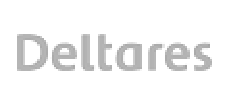
\includegraphics[width=0.6\textwidth]{image5} 
  \caption{Random wave angles are chosen using a random number generator and the cumulative distribution function of the directional spreading of the input spectrum}
  \label{fig:image5}
\end{figure}

Once the frequency and direction of each wave component has been selected, the amplitude Bi can be calculated by two dimensional interpolations across the 2D-input wave variance spectrum. A linear correction is made to the amplitudes of the wave components to ensure the integrated wave variance of the K components is the same as that of the input spectrum. The wave number \textit{k${}_{i}$} is determined using the dispersion relation, given the mean still water depth at the offshore boundary.

Equation \eqref{ZEqnNum661480} can now be used to generate a time series of the sea surface elevation at the offshore boundary. The envelope of the sea surface time series can be calculated using a Hilbert transform, the amplitude of which being a measure for the wave energy:

\begin{equation} \label{ZEqnNum899873} 
E_{\theta _{i} } \left(y,t\right)=\frac{1}{2} \rho gA_{\theta _{i} } \left(y,t\right) 
\end{equation} 

The particle velocity due to bound infragravity waves at the offshore boundary is calculated according to the expressions developed by \citet{Herbers1994}. It is stated that bound infragravity waves are generated by the interaction of two wave components with different frequencies. The frequency of the bound infragravity wave is given as:

\begin{equation} \label{2.23)} 
f_{3} =f_{2} -f_{1}  
\end{equation} 

In the equation above, the subscripts on the right hand side refer to the indices of interacting short wave pairs. In order to ensure positive interaction frequencies, indices should be ordered according to increasing frequency of the short wave components. It should be noted that two interacting wave components contribute to only one infragravity wave frequency. However, one infragravity wave frequency may be forced by many different wave component interactions.

Similarly, other properties of the bound infragravity wave can be deduced from the associated properties of the short wave components. The bound wave number, wave group velocity and wave phase are given as:

\begin{equation} \label{2.24)} 
k_{3} \equiv \left|\overrightarrow{k_{1} }-\overrightarrow{k_{2} }\right|=\sqrt{k_{1}^{2} +k_{2}^{2} -2k_{1} k_{2} \cos \left(\theta _{3} \right)}  
\end{equation} 

\begin{equation} \label{2.25)} 
c_{g3} =\frac{2\pi f_{3} }{k_{3} }  
\end{equation} 

\begin{equation} \label{ZEqnNum719840} 
\varphi _{3} =\varphi _{2} -\varphi _{1} +\pi  
\end{equation} 

Note that equation \eqref{ZEqnNum719840} is based on the assumption that the short wave groups and bound long waves are in equilibrium, and therefore are 180${}^\circ$ out of phase. The angle of the bound long wave can be found using the following relation:

\begin{equation} \label{2.27)} 
\theta _{3} =\arctan \left(\frac{k_{2} \sin \theta _{2} -k_{1} \sin \theta _{1} }{k_{2} \cos \theta _{2} -k_{1} \cos \theta _{1} } \right) 
\end{equation} 

The energy related to a bound infragravity wave with a specific frequency is given as \citep{VanDongeren2003}:

\begin{equation} \label{ZEqnNum984323} 
\begin{array}{l} {E_{3} \left(f_{3} \right)=2\int _{\Delta f}^{\infty }\int _{0}^{2\pi }\int _{0}^{2\pi }D^{2} \left(f+f_{3} ,-f,\left|\theta _{1} -\theta _{2} \right|+\pi \right)   } \\ {{\rm \; \; \; \; \; \; \; \; \; \; \; \; \; \; \; }\cdot E\left(f+f_{3} ,\theta _{1} \right)E\left(f,\theta _{2} \right)d\theta _{2} d\theta _{1} df} \end{array} 
\end{equation} 

Where in equation \eqref{ZEqnNum984323} the first term behind the triple integral is the interaction coefficient as defined by \citet{Herbers1994}. This interaction coefficient is determined through a perturbation expansion of the Bernouilli equation, details are in original publication. In the wave boundary condition module a modification of the interaction coefficient is implemented to convert the output to surface level elevation instead of bed level pressure:

\begin{equation} \label{2.29)} 
D_{surface} =D_{bed} \frac{\cosh \left(k_{3} h\right)}{\cosh \left(k_{1} h\right)\cosh \left(k_{2} h\right)}  
\end{equation} 

The amplitude of each bound wave can be found from the bound wave energy \citep{VanDongeren2003}:

\begin{equation} \label{2.30)} 
A_{3} =\sqrt{2E_{3} df}  
\end{equation} 

Where \textit{df} refers to the frequency resolution of the short waves, i.e. the frequency step used to generate all K frequency components around the peak of the short wave spectrum. 

A time series for the cross shore water flux across the offshore boundary is generated by means of an Inverse Fourier Transform:

\begin{equation} \label{2.31)} 
q_{x} (0,t)=IFFT\left[\sum _{i=1}^{K}\frac{A_{3,i} }{2}  e^{-i\varphi _{3,i} } c_{g3,i} \cos \theta _{3,i} \right] 
\end{equation} 

This cross-shore flux is phase-shifted along the offshore boundary as:

\begin{equation} \label{ZEqnNum107213} 
q_{x} (y,t)=IFFT\left[\sum _{i=1}^{K}\frac{A_{3,i} }{2}  e^{-i\varphi _{3,i} } c_{g3,i} \cos \theta _{3,i} e^{-ik_{y3,i} y} \right] 
\end{equation} 

The cross-shore flux \eqref{ZEqnNum107213} and the wave energy \eqref{ZEqnNum899873} are specified along the boundary.

\subparagraph{Procedure for converting spatially varying spectra to wave energy and bound long wave boundary conditions}

In cases where the user specifies more than one spectrum in space along the offshore boundary of the model, the procedure describe above to generate a boundary condition time series for one spectrum is modified to incorporate spatially varying boundary conditions.

Upon reading input, XBeach will determine the nearest numerical grid cell to the input location of each input spectrum. This location on the numerical grid is used in subsequent interpolation routines. 

At each input spectrum location, XBeach reads the input spectrum file (JONSWAP, SWAN or Vardens file) and maps the input spectrum to a common frequency-direction variance density grid. A copy of these individual spectra are used to generate a combined spectrum for the entire offshore boundary, which is used for the determination of the frequency, direction and phase of \textit{K} wave components (see previous section). This ensures that all important frequencies and directions are included in the offshore boundary conditions. The frequency and direction of all \textit{K} wave components remain constant along the offshore boundary.

The amplitude of each wave component at each grid point along the offshore boundary is determined by linear interpolation of the variance density corresponding to the frequency and direction of the wave component in the two neighboring input spectra. The distance used in the interpolation is the distance between the current grid point and the input spectra along the offshore edge of the model, rather than the absolute distance to the input spectra. Note that these distances only differ in case of a curvilinear grid. 

At each offshore grid point, a time series is now generated of the high-frequency sea surface elevation (Eq. \eqref{ZEqnNum661480}), using the local short wave amplitude and phase, and fixed period and direction of each wave component. The subsequent determination of the wave energy envelope and bound wave flux per offshore grid point is carried out in the same manner as for single-spectrum input.

\paragraph{Lateral wave boundary conditions}

For the lateral boundary conditions we make the following reasonable assumptions for the incoming  wave energy:

\begin{enumerate}
\item  In the default case, we assume that the alongshore gradient of the wave energy is zero; this means we copy the value of one row inside the domain to the boundary, for the directional bins where the direction is into the model domain;

\item  In other cases, we assume that the gradient along the crest of the wave group is zero. The direction of the crest is derived from the local mean wave direction and the values at the boundary are determined by interpolation between the two points on the row inside around a virtual point taken along the crest direction; in the figure, for example, the value at point (3,1) is interpolated from points (2,2) and (3,2).
\end{enumerate}

\begin{figure}[h]
  \centering
  \includegraphics[width=0.6\textwidth]{image6}
  \caption{Example of interpolation at the lateral boundary}
  \label{fig:image6}
\end{figure}

\begin{figure}[h]
  \centering
  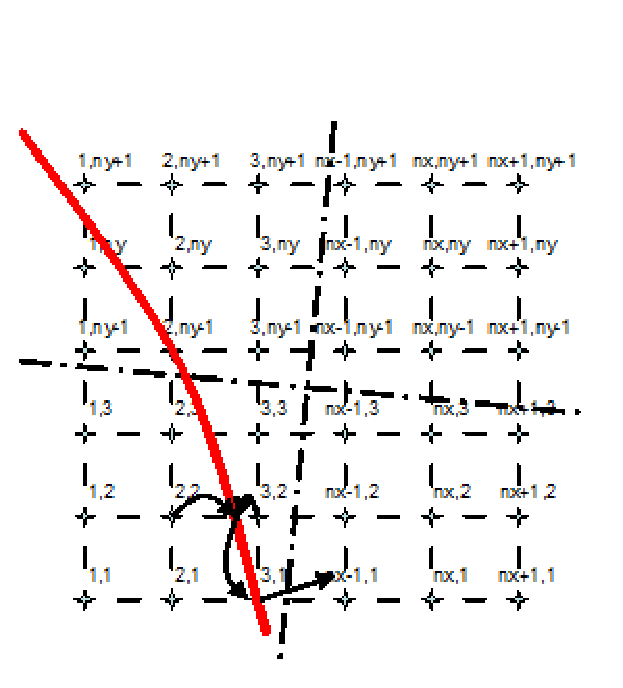
\includegraphics[width=0.6\textwidth]{image7}
  \caption{Example of interpolation at the lateral boundary}
  \label{fig:image7}
\end{figure}


\section{ Roller energy equation solver}

The roller energy balance is coupled to the wave action/energy balance where dissipation of wave energy serves as a source term for the roller energy balance. Similar to the wave action the directional distribution of the roller energy is taken into account whereas the frequency spectrum is represented by a single mean frequency. 

The roller energy balance is then given by:

\begin{equation} \label{2.33)} 
\frac{\partial S_{r} }{\partial t} +\frac{\partial c_{x} S_{r} }{\partial x} +\frac{\partial c_{y} S_{r} }{\partial y} +\frac{\partial c_{\theta } S_{r} }{\partial \theta } =-D_{r} +D_{w}  
\end{equation} 

with the roller energy in each directional bin represented by $S_{r} (x,y,t,\theta )$.The roller energy propagation speeds in x- and y-direction are given by:

\begin{equation} \label{2.34)} 
\begin{array}{l} {c_{x} (x,y,t,\theta )=c\cos (\theta )+u^{L} } \\ {c_{y} (x,y,t,\theta )=c\sin (\theta )+v^{L} } \end{array} 
\end{equation} 

where $\Theta$ represents the angle of incidence with respect to the x-axis.  If wave-current interaction is turned off (\textit{wci=0}) then the last terms in either equation are not taken into account.

The propagation speed in $\theta $-space is identical to the expression used for the wave energy density propagation, (eq. \eqref{ZEqnNum944441}, thus assuming that waves and rollers propagate in the same direction. The phase velocity is obtained from linear wave theory:

\begin{equation} \label{2.35)} 
c=\frac{\sigma }{k}  
\end{equation} 

The total roller energy dissipation is given by \citep{Reniers2004a}:

\begin{equation} \label{2.36)} 
\bar{D}_{r} =\frac{2g\beta _{r} E_{r} }{c}  
\end{equation} 

which combines concepts by \citet{Deigaard1993} and \citet{Svendsen1984}

Next the total roller dissipation,$\bar{D}_{r} $, is distributed proportionally over the wave directions:

\begin{equation} \label{2.37)} 
D_{r} (x,y,t,\theta )=\frac{S_{r} (x,y,t,\theta )}{E_{r} (x,y,t)} \bar{D}_{r} (x,y,t) 
\end{equation} 

This closes the set of equations for the roller energy balance. 

The roller contribution to radiation stress is given by:

\begin{equation} \label{2.38)} 
\begin{array}{l} {S_{xx,r} (x,y,t)=\int \cos ^{2} \theta S_{r} d\theta  } \\ {S_{xy,r} (x,y,t)=S_{yx,r} (x,y,t)=\int \sin \theta \cos \theta S_{r}  d\theta } \\ {S_{yy,r} (x,y,t)=\int \sin ^{2} \theta S_{r} d\theta  } \end{array} 
\end{equation} 

These roller radiation stress contributions are added to the wave-induced radiation stresses (eq. \eqref{ZEqnNum727357} to calculate the wave forcing utilizing the radiation stress tensor:  

\begin{equation} \label{2.39)} 
\begin{array}{l} {F_{x} (x,y,t)=-\left(\frac{\partial S_{xx,w} +S_{xx,r} }{\partial x} +\frac{\partial S_{xy,w} +S_{xy,r} }{\partial y} \right)} \\ {F_{y} (x,y,t)=-\left(\frac{\partial S_{xy,w} +S_{xy,r} }{\partial x} +\frac{\partial S_{yy,w} +S_{yy,r} }{\partial y} \right)} \end{array} 
\end{equation} 

\section{ Shallow water equations solver}
\subsection{ Depth-averaged equations}

For the low-frequency and mean flows we use the shallow water equations. To account for the wave induced mass-flux and the subsequent (return) flow these are cast into a depth-averaged Generalized Lagrangian Mean (GLM) formulation \citep{AndrewsMcIntyre1978, Walstra2000}. In such a framework, the momentum and continuity equations are formulated in terms of the Lagrangian velocity, \textit{u${}^{L}$}, which is defined as the distance a water particle travels in one wave period, divided by that period. This velocity is related to the Eulerian velocity (the short-wave-averaged velocity observed at a fixed point) by:

\begin{equation} \label{2.40)} 
u^{L} =u^{E} +u^{S} \quad and\quad v^{L} =v^{E} +v^{S}  
\end{equation} 

Here \textit{u${}^{S}$} ,\textit{ v${}^{S}$} represents the Stokes drift in x- and y-direction respectively \citep{Phillips1977}:

\begin{equation} \label{2.41)} 
u^{S} =\frac{E_{w} \cos \theta }{\rho hc} \quad and\quad v^{S} =\frac{E_{w} \sin \theta }{\rho hc}  
\end{equation} 

where the wave-group varying short wave energy and direction are obtained from the wave-action balance (eq.\eqref{ZEqnNum711560}. The resulting GLM-momentum equations are given by:  

\begin{equation} \label{2.42)} 
\frac{\partial u^{L} }{\partial t} +u^{L} \frac{\partial u^{L} }{\partial x} +v^{L} \frac{\partial u^{L} }{\partial y} -f\, v^{L} \, -\, \nu _{h} \left(\frac{\partial ^{2} u^{L} }{\partial x^{2} } +\frac{\partial ^{2} u^{L} }{\partial y^{2} } \right)=\frac{\tau _{sx} }{\rho h} -\frac{\tau _{bx}^{E} }{\rho h} -g\frac{\partial \eta }{\partial x} +\frac{F_{x} }{\rho h}  
\end{equation} 

\begin{equation} \label{2.43)} 
\frac{\partial v^{L} }{\partial t} +u^{L} \frac{\partial v^{L} }{\partial x} +v^{L} \frac{\partial v^{L} }{\partial y} +f\, u^{L} \, -\, \nu _{h} \left(\frac{\partial ^{2} v^{L} }{\partial x^{2} } +\frac{\partial ^{2} v^{L} }{\partial y^{2} } \right)=+\frac{\tau _{sy} }{\rho h} -\frac{\tau _{by}^{E} }{\rho h} -g\frac{\partial \eta }{\partial y} +\frac{F_{y} }{\rho h}  
\end{equation} 

\begin{equation} \label{2.44)} 
\frac{\partial \eta }{\partial t} +\frac{\partial hu^{L} }{\partial x} +\frac{\partial hv^{L} }{\partial y} =0 
\end{equation} 

Here $\tau _{bx} ,\tau _{by} $ are the bed shear stresses, $\eta $ is the water level, $F_{x} $,$F_{y} $ are the wave-induced stresses, $\nu _{t} $is the horizontal viscosity and \textit{f} is the Coriolis coefficient. The bottom shear stress terms are calculated with the Eulerian velocities as experienced by the bed:

\begin{equation} \label{2.45)} 
u^{E} =u^{L} -u^{S} \quad and\quad v^{E} =v^{L} -v^{S}  
\end{equation} 

and not with the GLM velocities. Also, the boundary condition for the flow computations are expressed in functions of (u${}^{L}$ , v${}^{L}$ ) and not (u${}^{E}$, v${}^{E}$).

\paragraph{Smagorinsky viscosity}
TEXTO BE INSERTED

\paragraph{White-Colebrook bottom roughness}
TEXT TO BE INSERTED

\subsection{ Quasi-3D equations (advanced option)}
NOT OPERATIONAL YET TO BE INSERTED

\subsection{ Flow boundary conditions}
\paragraph{Offshore flow boundary conditions}

\underbar{Usually, }the offshore boundary is an artificial boundary which has no physical meaning. On the offshore boundary wave and flow conditions are imposed. In the domain waves and currents will be generated which need to pass through the offshore boundary to the deep sea with minimal reflection. One way to do this is to impose a weakly reflective-type boundary condition. 

The options are:

\begin{tabular}{|p{0.5in}|p{0.8in}|p{2.6in}|} \hline 
front & abbreviated name & description \\ \hline 
0 & abs1d & absorbing-generating (weakly-reflective) boundary in 1D \\ \hline 
1 & abs2d & same, in 2D (default setting) \\ \hline 
2 & wall & no flux wall \\ \hline 
3 & wlevel & water level specification (from file) \\ \hline 
4 & nonh\_1d & boundary condition for nonhydrostatic option \\ \hline 
\end{tabular}

\subparagraph{1D absorbing-generating boundary condition}

In XBeach, there are two options with regard to the offshore absorbing-generating boundary condition. With the parameter setting ``front = 0'' a simple one-dimensional radiating boundary condition is activitated. 

It reads:

\begin{equation} \label{ZEqnNum247802} 
{\rm u=}\left({\rm 1+}\frac{\sqrt{{\rm g}\, {\rm h}} }{{\rm c}_{{\rm g}} } \right){\rm u}_{{\rm i}} {\rm +}\bar{{\rm u}}{\rm -}\sqrt{\frac{{\rm g}}{{\rm h}} } {\rm (z}_{{\rm s}} {\rm -z}_{{\rm s0}} {\rm )} 
\end{equation} 

Where u${}_{i}$ is the incoming particle velocity and z${}_{s}$ is the surface elevation of the incoming bound long wave, and z${}_{s}$${}_{0}$ is the mean water level (averaged over many wave groups), $\bar{u}$is the mean velocity (current). This boundary condition assumes all incoming and outgoing waves propagate normal to the boundary. It is therefore only useful for 1D (flume like) simulations.

\subparagraph{2D absorbing-generating boundary condition}

With option ``front = 1'' (default value) the formulation by \citet{VanDongeren1997} is activated which in turn is based on \citet{Verboom1981} and is based on the Method of Characteristics. This boundary condition allows for obliquely-incident and reflected waves, and is therefore suited for 1D and 2D computations. 

The boundary conditions satisfy the following two necessary conditions:  

\begin{enumerate}
  \item  the region outside the computation domain can influence the motion within the domain only through the incident (long) waves and through the currents along the boundaries; and
  \item  the (long) waves propagating out of the computational domain must be allowed to freely propagate through the open-ocean offshore boundary with minimal reflection.  
\end{enumerate}

By placing the open boundaries carefully, one can achieve weak local forcing near these boundaries. In practice this means that the offshore boundary is placed in sufficiently deep water, i.e. outside the shoaling zone. Then the dominant terms in the continuity and momentum equations near these boundaries are the nonlinear shallow water equation.s 

For the general case of an arbitrary angle $\upsilon $ between the boundary at a point and the coordinate axes, one can follow the work of \citet{Abbott1979} and \citet{Verboom1981} to derive the governing equations, which are valid for an arbitrary angle $\upsilon $ between the coordinate axes and the model boundary (Figure 2.5a).

\begin{figure}[h]
  \centering
  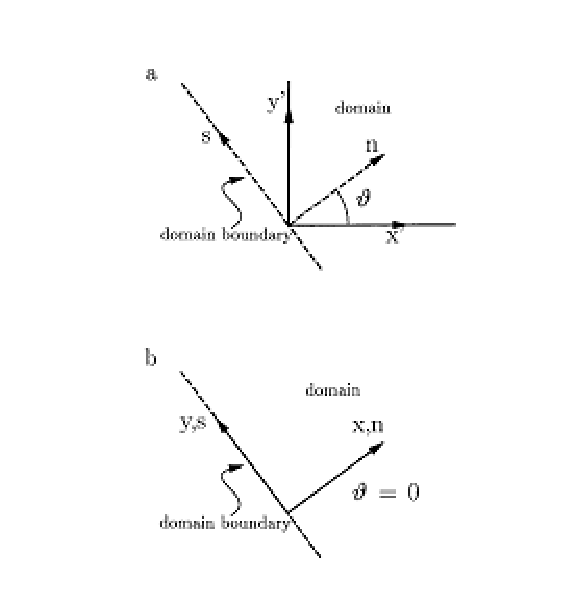
\includegraphics[width=0.6\textwidth]{image9} 
  \caption{Coordinate system (a) for arbitrary angle $\upsilon $ between domain boundary and x-axis$;$ (b) for $\upsilon $=0}
  \label{fig:image9}
\end{figure}

The derivation becomes simplified if the coordinate system is defined in a way the the x-axis is normally inward to the seaward boundary of the rectangular domain, which sets $\upsilon $=0 (Figure 2.5b).  The governing equations derived following \citet{Abbott1979} and \citet{Verboom1981} then simplify to:

\begin{equation} \label{ZEqnNum327963} 
\frac{\partial \beta ^{-} }{\partial t} =-(u-c)\frac{\partial \beta ^{-} }{\partial x} -v\frac{\partial \beta ^{-} }{\partial y} +c\frac{\partial v}{\partial y} +g\frac{\partial h_{0} }{\partial x} +F_{\beta ^{-} }  
\end{equation} 

\begin{equation} \label{2.48)} 
\frac{\partial \beta ^{+} }{\partial t} =-(u+c)\frac{\partial \beta ^{+} }{\partial x} -v\frac{\partial \beta ^{+} }{\partial y} -c\frac{\partial v}{\partial y} +g\frac{\partial h_{0} }{\partial x} +F_{\beta ^{+} }  
\end{equation} 

\begin{equation} \label{ZEqnNum829814} 
\frac{\partial \gamma }{\partial t} =-u\frac{\partial \gamma }{\partial x} -v\frac{\partial \gamma }{\partial y} -g\frac{\partial \eta }{\partial y} +F_{\gamma }  
\end{equation} 

Where, \textit{F} includes all local forcing and friction terms for the motion, \textit{c} is the wave celerity, and \textit{h${}_{0}$} is the still water depth.  The Riemann variable \textit{$\beta $}${}^{-}$ is defined as: 

\begin{equation} \label{ZEqnNum437792} 
\beta ^{-} =u-2c=u-2\sqrt{g(h_{0} +\eta )}  
\end{equation} 

Here \textit{u} is the depth-averaged velocity. The Riemann variable $\beta $+ is similarly defined as $\beta^{+} = u + 2c$. The $\gamma$-equation is the y-momentum equation, which has the Riemann variable:

\begin{equation} \label{2.51)} 
\gamma =v 
\end{equation} 

The definition sketch in Figure 2.6 shows that  $\beta $- propagates in the negative \textit{x}-direction, $\beta $+ propogates in the positive \textit{x}-direction, and $\gamma $ in the \textit{y}-direction. 

The forcing terms, \textit{F}, in equations \eqref{ZEqnNum327963}-\eqref{ZEqnNum829814} originate from the right-hand side of the nonlinear shallow water equations, which imply that $\beta $- , $\beta $+, and $\gamma $ are variables rather than constants.  

\begin{figure}[h]
  \centering
  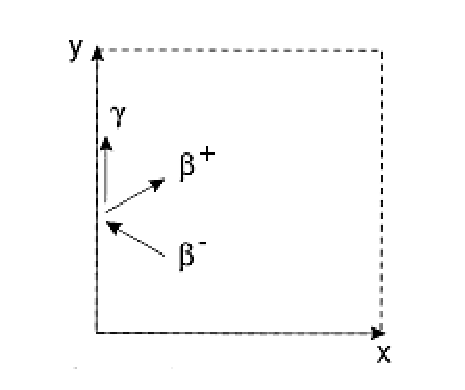
\includegraphics[width=0.6\textwidth]{image11} 
  \caption{Definition sketch of the characteristics}
  \label{fig:image11} 
\end{figure}

The offshore boundary conditions uses the outgoing $\beta $- variant which contains information about the waves leaving the domain and the $\gamma $ variant which propagates along the boundary. The latter is extra information which we will use to estimate the direction of the outgoing wave which is the innovation in \citet{VanDongeren1997}.

The procedure is as follows: during the computation, at time step \textit{n}, we know the values of $\eta^n$ and the total velocities $(u^n,v^n)$ at all points in the domain.  The incoming wave is specified along the open boundaries through the \textit{x} and \textit{y} components of the particle velocities of the incident wave $(u_{in},v_{in})$.  The numerical integration of nonlinear shallow water equations will provide the values of the total $\eta$, \textit{u}, and \textit{v} for the interior points in the domain at time step \textit{n+1}, and then the equivalent total (incoming plus outgoing) values need to be determined along the boundaries at \textit{n+1}.  In other words, given the incoming wave, the outgoing wave needs to be determined. 

In XBeach the lowest-order derived equations are implemented for the weakly reflective boundary conditions, with x=0 at the boundary.  The outgoing wave angle (\textit{$\theta $${}_{r}$})  and velocity in the \textit{x}-direction (\textit{u${}_{r}$})  are solved iteratively.  For specifics on this derivation we refer to \citet{VanDongeren1997}, the shorter outline is given below

The \textit{$\beta $-} is updated along the boundary only through \eqref{ZEqnNum327963} which discretized in XBeach (similarly as the \textit{x}-momentum equation) reads 

\begin{equation} \label{2.52)} 
\frac{\beta _{i,j}^{n+1} -\beta _{i,j}^{n} }{\Delta t} =-\left(u-c\right)\frac{\partial \beta }{\partial x} _{i,j}^{n} -v\frac{\partial \beta }{\partial y} _{i,j}^{n} +c\frac{\partial v}{\partial y} _{i,j}^{n} +g\frac{h_{{\rm i+1,j}}^{n} -h_{{\rm i,j}}^{{\rm n}} }{x_{{\rm i+1,j}} -x_{{\rm i,j}} } +\frac{F_{x,i,j} }{\rho h_{u,i,j} }  
\end{equation} 

And is thus known at the time level \textit{n+1}. We can then solve for the outgoing velocity \textit{u${}_{r}$} by expanding the Riemann variant \eqref{ZEqnNum437792} to lowest order as

\begin{equation} \label{ZEqnNum940080} 
\beta ^{-} =u-2\sqrt{g(h_{0} +\eta )} =u-2\sqrt{gh_{0} } \left(1+\frac{1}{2} \frac{\eta }{h_{0} } \right) 
\end{equation} 

We further have the identities

\begin{equation} \label{2.54)} 
\begin{array}{l} {u=u_{i} +u_{r} +\bar{u}} \\ {\eta =\eta _{i} +\eta _{r} } \\ {u_{i} =c_{g} \eta _{i} \, \cos \theta _{i} } \\ {u_{r} =-\sqrt{gh_{0} } \, \eta _{r} \, \cos \theta _{r} } \end{array} 
\end{equation} 

where the last two identities assume waves propagating with constant form. The incoming bound wave propagates at the group speed and the reflected wave at the free shallow water celerity,  where \textit{$\theta $${}_{i}$} and \textit{$\theta $${}_{r}$} are the angles of the incoming (known) wave and the outgoing (yet unknown) wave, relative to the x=0 boundary. $\bar{u}$is the mean current. Inserting these identities into \eqref{ZEqnNum940080} and re-arranging gives:

\begin{equation} \label{ZEqnNum523309} 
u_{r} =\left(\frac{\cos \theta _{r} }{\cos \theta _{r} +1} \right)\left[\beta ^{-} -\bar{u}+2\sqrt{gh_{0} } -u_{i} \left(\frac{c_{g} \cos \theta _{i} -\sqrt{gh_{0} } }{c_{g} \cos \theta _{i} } \right)\right] 
\end{equation} 

All the terms on the right hand side are known except for $\theta $r which can be solved from the $\gamma $ = v variant as:

\begin{equation} \label{ZEqnNum431229} 
\theta _{r} =\arctan \left(\frac{u_{r} }{v_{r} } \right)=\arctan \left(\frac{u_{r} }{v-v_{i} -\bar{v}} \right) 
\end{equation} 

Eqs. \eqref{ZEqnNum523309} and \eqref{ZEqnNum431229} are then solved iteratively to yield both \textit{u${}_{r}$}${}_{ }$and \textit{$\theta $${}_{r}$}. The final boundary condition is then the total velocity u\textit{ u = u${}_{i }$+ u${}_{r}$} + $\bar{u}$at the boundary at the time level \textit{n+1}.

\paragraph{Wall boundary condition}

This boundary condition type is activated using ``front =2'' and is a simple no flux boundary condition.

\paragraph{Water level boundary condition}

This boundary sets the water level at a prescribed value. This can be constant or time-varying, see description of tide varying surge in Chapter 5. With this option the outgoing long waves are not absorbed. 

\subparagraph{Non-hydrostatic boundary condition}

This option is to be used with the non-hydrostatic mode, see Appendix

\paragraph{Bay-side flow boundary condition}

In many cases, the onshore boundary will be a land boundary. In some case the ``onshore'' will be a bay behind a barrier island. In that case it is possible to specify a number of boundary conditions.

The options are:

\begin{tabular}{|p{0.5in}|p{0.8in}|p{2.6in}|} \hline 
\textbf{back} & abbreviated name & description \\ \hline 
0 & wall & no flux wall \\ \hline 
1 & abs1d & absorbing-generating (weakly-reflective) boundary in 1D \\ \hline 
2 & abs2d & same, in 2D (default setting) \\ \hline 
3 & wlevel & water level specification (from file) \\ \hline 
\end{tabular}

\subparagraph{1D absorbing boundary condition }

This boundary condition type is activated using ``back = 0' and is analoguous to \eqref{ZEqnNum247802}without the possibility of specifying an incoming particle velocity.

\subparagraph{Wall boundary condition}

This boundary condition type is activated using ``back =1'' and is a simple no flux boundary condition

\subparagraph{2D absorbing boundary condition (default)}

This boundary condition type is activated using ``back = 2'' and is analoguous to the absorbing-generating boundary condition by \citet{VanDongeren1997}, but without the incoming particle velocities (so 2D absorbing only). 

\paragraph{Water level boundary condition}

See above.

\paragraph{Lateral flow boundary conditions}

\begin{figure}[h]
  \centering
  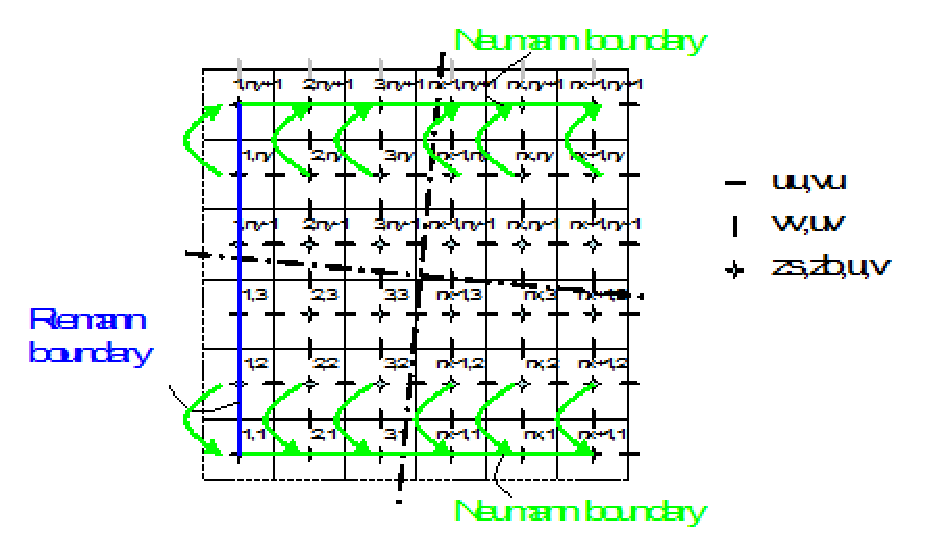
\includegraphics[width=0.6\textwidth]{image16}
  \caption{Stencil for Neumann-type boundary conditions}
  \label{fig:image16}
\end{figure}

\subparagraph{Neumann boundaries (default)}

Lateral boundaries are the boundaries perpendicular to the coastline. Usually these are artificial, because the model domain is limited but the physical coast will continue. At these boundaries we need to prescribe information about the area beyond the numerical model domain in such a way that the boundary condition does not influence the results in an adverse way. The best way to do this is to prescribe so-called ``no-gradient'' or Neumann boundaries, which state that there is locally no change in surface elevation and velocities.

These boundary conditions are activitate using ``left = 0'' or equivalently ``left=neumann'' and/or ``right = 0'' or equivalently ``right=neumann''), where the longshore water level gradient is prescribed. The alongshore gradient is prescribed by the difference in specified water levels at the offshore corner points, divided by the alongshore length of the domain. 

This type of Neumann boundary condition has been shown to work quite well with (quasi-) stationary situations, where the coast can be assumed to be uniform alongshore outside the model domain. So far we have found that also in case of obliquely incident wave groups this kind of boundary conditions appears to give reasonable results, though rigorous testing still has to be done. The implementation consists of copying water levels from row 2 to row 1 and from row \textit{ny} to row \textit{ny+1}, and doing the same for the cross-shore (along-boundary) velocities. The alongshore velocities can now be computed from row 1 through row \textit{ny}; no additional boundary conditions are required for the alongshore velocity.

Simple no-flux boundary conditions (walls) can be set using ``left = 1'' (or left = wall) and/or ``right = 1'' or ``right = wall''. Wall boundary conditions are preferred over Neumann boundary conditions in 1D (cross-shore) models.


\section{Sediment transport}
\paragraph{Advection-diffusion scheme}

The sediment transport is modeled with a depth-averaged advection diffusion equation \citep{Galappatti1985}:

\begin{equation} \label{2.57)} 
\frac{\partial hC}{\partial t} +\frac{\partial hCu^{E} }{\partial x} +\frac{\partial hCv^{E} }{\partial y} +\frac{\partial }{\partial x} \left[D_{h} h\frac{\partial C}{\partial x} \right]+\frac{\partial }{\partial y} \left[D_{h} h\frac{\partial C}{\partial y} \right]=\frac{hC_{eq} -hC}{T_{s} }  
\end{equation} 

where \textit{C }represents the depth-averaged sediment concentration which varies on the wave-group time scale, and \textit{D${}_{h}$} is the sediment diffusion coefficient. The entrainment of the sediment is represented by an adaptation time \textit{T${}_{s}$}, given by a simple approximation based on the local water depth, \textit{h}, and sediment fall velocity \textit{w${}_{s}$}:

\begin{equation} \label{2.58)} 
T_{s} =\max \left(0.05\frac{h}{w_{s} } ,0.2\right)\; s 
\end{equation} 

where a small value of \textit{T${}_{s}$ }corresponds to nearly instantaneous sediment response. The entrainment or deposition of sediment is determined by the mismatch between the actual sediment concentration, \textit{C}, and the equilibrium concentration, \textit{C${}_{eq}$}, thus representing the source term in the sediment transport equation. 

The bed-updating is discussed next. Based on the gradients in the sediment transport the bed level changes according to:

\begin{equation} \label{2.59)} 
\frac{\partial z_{b} }{\partial t} +\frac{f_{mor} }{\left(1-p\right)} \left(\frac{\partial q_{x} }{\partial x} +\frac{\partial q_{y} }{\partial y} \right)=0 
\end{equation} 

where \textit{p }is the porosity, $f_{mor} $ is a morphological acceleration factor of O(1-10) \citep[e.g.][]{Reniers2004a}  and\textit{ q${}_{x}$} and \textit{q${}_{y}$} represent the sediment transport rates in \textit{x}- and \textit{y}-direction respectively, given by:

\begin{equation} \label{2.60)} 
q_{x} (x,y,t)=\left[\frac{\partial hCu^{E} }{\partial x} \right]+\left[\frac{\partial }{\partial x} \left[D_{h} h\frac{\partial C}{\partial x} \right]\right] 
\end{equation} 

and

\begin{equation} \label{2.61)} 
q_{y} (x,y,t)=\left[\frac{\partial hCv^{E} }{\partial y} \right]+\left[\frac{\partial }{\partial y} \left[D_{h} h\frac{\partial C}{\partial y} \right]\right] 
\end{equation} 

To account for bed-slope effects on sediment transport a bed-slope correction factor f${}_{slope}$ is introduced. 

\paragraph{Transport formulations}

The equilibrium sediment concentration can be calculated with various sediment transport formulae. At the moment the sediment transport formulation of Soulsby-van Rijn \citep{Soulsby1997} has been implemented. The \textit{C${}_{eq}$} is then given by:

\begin{equation} \label{2.62)} 
C_{eq} =\frac{A_{sb} +A_{ss} }{h} \left(\left(|u^{E} |^{2} +0.018\frac{u_{rms}^{2} }{C_{d} } \right)^{0.5} -u_{cr} \right)^{2.4} (1-\alpha _{b} m) 
\end{equation} 

where sediment is stirred by the Eulerian mean and infragravity velocity in combination with the near bed short wave orbital velocity, \textit{u${}_{rms}$}. In the default mode, the sediment is stirred due to mean and infragravity velocities. By setting \textit{lws = 0} the mean component can be excluded. The shortwave stirring can be turned off by setting \textit{sws = 0}. By default \textit{sws = 1}. The \textit{u${}_{rms}$} obtained from the wave-group varying wave energy using linear wave theory as

\begin{equation} \label{2.63)} 
{\rm u}_{{\rm rms}} =\frac{\pi H_{rms} }{T_{rep} \sqrt{2} \sinh (kh+\delta H_{rms} )}  
\end{equation} 

The combined mean/infragravity and orbital velocity have to exceed a threshold value, \textit{u${}_{cr}$}, before sediment is set in motion. The drag coefficient, \textit{C${}_{d}$}, is due to flow velocity only (ignoring short wave effects). To account for bed-slope effects on the equilibrium sediment concentration a bed-slope correction factor is introduced, where the bed-slope is denoted by \textit{m} and $\alpha _{b} $ represents a calibration factor. The bed load coefficients \textit{A${}_{sb}$ }and the suspended load coefficient \textit{A${}_{ss}$} are functions of the sediment grain size, relative density of the sediment and the local water depth (see \citet{Soulsby1997} for details). Note that the transport model does not contain transport contributions related to wave skewness.

The Soulsby-Van Rijn formulation is not strictly valid for sheet flow conditions. If applied in high velocity situations, the formulation as used in XBeach leads to unrealistically high sediment transport rates. In order to compensate this, steady flow velocities used to mobilize sediment are limited by an upper-bound Shields parameter for the start of sheet flow 
\[(\theta sf = 0.8 -- 1.0):\] 

\begin{equation} \label{2.64)} 
u_{flow,stirring}^{2} =\min \left(\left(u^{E} \right)^{2} +\left(v^{E} \right)^{2} ,\theta _{sf} \frac{gD_{50} \Delta }{c_{f} } \right) 
\end{equation} 

This approach assumes that in sheet flow conditions higher velocities lead to higher sediment transport rates, but not to higher equilibrium sediment concentrations, which is not necessarily correct. However, the assumption does cause sediment discharge under sheet flow conditions to become a linear function of flow discharge, which is in line with \citet{Kobayashi1996}.

\subsection{ Wave asymmetry}

The wave asymmetry enters the advection-diffusion equation, repeated here:

\begin{equation} \label{2.65)} 
\frac{\partial hC}{\partial t} +\frac{\partial hCu_{AV} }{\partial x} +\frac{\partial hCv_{AV} }{\partial y} +\frac{\partial }{\partial x} \left[D_{h} h\frac{\partial C}{\partial x} \right]+\frac{\partial }{\partial y} \left[D_{h} h\frac{\partial C}{\partial y} \right]=\frac{hC_{eq} -hC}{T_{s} }  
\end{equation} 

where

\begin{equation} \label{2.66)} 
\begin{array}{l} {u_{AV} =V_{W} \cos \theta _{m} +u^{E} } \\ {v_{AV} =V_{W} \sin \theta _{m} +v^{E} } \end{array} 
\end{equation} 

with $\theta $m is the mean wave angle and 

\begin{equation} \label{2.67)} 
V_{W} =\gamma _{ua} u_{rms} \left(S_{k} -A_{s} \right) 
\end{equation} 

is the velocity amplitude, with $\gamma $ua the free parameter, keyword facua. and 

\begin{equation} \label{2.68)} 
\begin{array}{l} {S_{k} =\frac{0.79}{1+\exp \frac{-0.61-\log U_{r} }{-0.35} } \cos \left(-\frac{\pi }{2} +\frac{\pi }{2} \tanh \left(0.64/U_{r}^{0.60} \right)\right)} \\ {A_{s} =\frac{0.79}{1+\exp \frac{-0.61-\log U_{r} }{-0.35} } \sin \left(-\frac{\pi }{2} +\frac{\pi }{2} \tanh \left(0.64/U_{r}^{0.60} \right)\right)} \end{array} 
\end{equation} 

the skewness and asymmetry as parameterized as a function of the Ursell number by Ruessink  and Van Rijn.

\section{ Morphological updating}
\subsection{ Avalanching}

To account for the slumping of sandy material during storm-induced dune erosion avalanching is introduced to update the bed-evolution. Avalanching is introduced when a user-defined critical bed-slope (keywords: wetslp and dryslp) is exceeded:

\begin{equation} \label{2.69)} 
\left|\frac{\partial z_{b} }{\partial x} \right|>m_{cr}  
\end{equation} 

Where the estimated bed slope is given by:

\begin{equation} \label{2.70)} 
\frac{\partial z_{b} }{\partial x} =\frac{z_{b,i+1,j} -z_{b,i,j} }{\Delta x}  
\end{equation} 

The bed-change within one time step is then given by:

\begin{equation} \label{2.71)} 
\begin{array}{l} {\Delta z_{b} =\min \left(\, \, \, \, \left(\left|\frac{\partial z_{b} }{\partial x} \right|-m_{cr} \right)\Delta x,\, \, \, \, 0.05\Delta t\right)\quad ,\frac{\partial z_{b} }{\partial x} >0} \\ {\Delta z_{b} =\max \left(-\left(\left|\frac{\partial z_{b} }{\partial x} \right|-m_{cr} \right)\Delta x,-0.05\Delta t\right)\quad ,\frac{\partial z_{b} }{\partial x} <0} \end{array} 
\end{equation} 

Where a threshold of 0.05 m/s has been introduced to prevent the generation of large shockwaves. The corresponding bed update is given by:

\begin{equation} \label{2.72)} 
\begin{array}{l} {z_{b,i,j}^{n+1} \, \, \, \, =z_{b,i,j}^{n} \, \, \, \, +\Delta z_{b,i,j} } \\ {z_{b,i+1,j}^{n+1} =z_{b,i+1,j}^{n} -\Delta z_{b,i,j} } \end{array} 
\end{equation} 

To account for continuity, e.g. when sand is deposited within the wet part of the domain, the water level is also updated:

\begin{equation} \label{2.73)} 
\begin{array}{l} {z_{s,i,j}^{n+1} \, \, \, \, =z_{s,i,j}^{n} \, \, \, \, +\Delta z_{b,i,j} } \\ {z_{s,i+1,j}^{n+1} =z_{s,i+1,j}^{n} -\Delta z_{b,i,j} } \end{array} 
\end{equation} 

Similar expressions are used for the subsequent avalanching in the y-direction. Here we consider that inundated areas are much more prone to slumping and therefore we apply separate critical slopes for dry and wet points; default values are 1 and 0.3, respectively. The former value is consistent with the equilibrium profile according to \citet{Vellinga1986}; it is higher than the angle of natural repose and must be seen as an average slope observed after dune erosion, where some stretches may exhibit vertical slopes and other, drier parts may have slumped further. The underwater critical slope is much lower, and our estimate is based on the maximum underwater slopes we have observed in experiments, e.g. the Zwin test (see below) and tests carried out at PlaceNameplaceOregon PlaceTypeState PlaceTypeUniversity with initially rather steep profiles.

When the critical slope between two adjacent grid cells is exceeded, sediment is exchanged between these cells to the amount needed to bring the slope back to the critical slope. This exchange rate is limited by a user-specified maximum avalanching transport rate, which for sandy environments is usually set so high as to have no influence on the outcome, while ensuring numerical stability. 

In our model simulations, the avalanching mechanism is typically triggered when a high infragravity wave reaches the dune front and partly inundates it. The critical underwater slope is suddenly exceeded and the two grid cells at the dune foot are adjusted during the first timestep when this happens. In subsequent timesteps a chain reaction may take place both in points landward, where now the critical dry slope may be exceeded because of the lowering of the last wet point, and in points seaward, where now the critical wet slope may be exceeded. As a result, sediment is brought from the dry dune into the wet profile, where it is transported further seaward by undertow and infragravity backwash. An essential difference with similar procedures in other dune erosion models is the fact that avalanching is only applied between adjacent grid cells, rather than extrapolating profile behaviour well beyond the wet domain. This is made possible by explicitly resolving the long-wave swash motions. Another big advantage with respect to existing procedures is that the simple avalanching algorithm is readily applied in two dimensions.

\subsection{ Morfac options}

The morfac is the morphological acceleration factor that speeds up the morphological time scale relative to the hydrodynamic timescale. It means that if you have a simulation of 10 minutes with a morfac of 6 you effectively simulate the morphological evolution over one hour. There are now two ways in which you can input the time-varying parameters in combination with morfac; this is governed by the input option morfacopt.

\textbf{morfacopt=1} 

All times are prescribed on input in morphological time. If you apply a morfac all input timeseries and other time parameters are divided internally by morfac. This way, you can specify all timeseries as real times, and vary the morfac without changing the rest of the input files. A typical application is that you run over a storm of some days and specify time-varying water level and wave conditions. If you now specify a morfac of 6, the model just runs for 10 (hydrodynamic) minutes each hour, during which the bottom changes per step are multiplied by a factor 6. This of course saves a factor of 6 in computation time.

An important thing to note is that the can only be done as long as the water level changes that are now accelerated by morfac do not modify the hydrodynamics too much. This is the case if the tide is perpendicular to the coast and the vertical variations do not lead to significant currents. If you have an alongshore tidal current, as is the case in shallow seas, you cannot apply this method because you would affect the inertia terms and thus modify the tidal currents.

\textbf{morfacopt=0}

In this new option the philosophy is different: you run the model over, say, a tidal cycle and apply the morfac without modifying the time parameters. This means you leave all the hydrodynamic parameters unchanged and just exaggerate what happens within a tidal cycle. As long as the evolution over a single tidal cycle is limited, the mean evolution over a tidal cycle using a morfac is very similar to running morfac tidal cycles without morfac. See \citet{Roelvink2006} for a more detailed description of this approach. This method is more appropriate for longer-term simulations with not too extreme events.

\section{ Multiple sediment fractions (advanced option)}

To model the overwash deposits at barrier islands during extreme conditions XBEACH has been extended with a multiple sediment class formulation. This allows for the tracking of sediment but also for assigning different sediment characteristics such as grain size diameter, fall velocity, mobility, etc. For each sediment class, \textit{i}, the equilibrium sediment concentration, $C_{eq}^{*}(i)$, is calculated according to the Soulsby-van Rijn formulation, see equation \eqref{GrindEQ__2_59_} .

The actual concentration then depends on the mismatch with the equilibrium concentration in combination with the available fraction at that location. It is assumed that a top-layer of 10 cm depth is readily available for sediment pick-up. So based on the fractions of the various sediment classes present in the top-layer the equilibrium concentration per sediment class can be expressed as:

\begin{equation} \label{2.74)} 
c_{eq} (i)=frc(i,1)c_{eq}^{*} (i) 
\end{equation} 

Where the index \textit{1} refers to the top layer and frc the fraction of a specific sediment class.  Next the advection-diffusion equation (see eq. 2.54) is solved independently for the different sediment classes leading to class dependent sediment transport rates, $S_i$, from which the bottom changes per sediment class, $\Delta z_i$, can be derived:

\begin{equation} \label{2.75)} 
\Delta z_{i} =\frac{\Delta t}{1-n_{p} } \left[\frac{\partial S_{i,x} }{\partial x} +\frac{\partial S_{i,y} }{\partial y} \right] 
\end{equation} 

Changes in fractional composition of the sediment classes in the top-layer due to sediment deposition are then calculated by:

\begin{equation} \label{2.76)} 
frc^{n+1} (i,1)=\frac{\Delta z_{i} }{D_{z} } +\frac{D_{z} -\Delta z}{D_{z} } frc^{n} (i,1) 
\end{equation} 

Given dz $<$= Dz, else:

\begin{equation} \label{2.77)} 
frc^{n+1} (i,1)=\frac{\Delta z_{i} }{\Delta z}  
\end{equation} 

And similarly for erosion:

\begin{equation} \label{2.78)} 
frc^{n+1} (i,1)=\frac{\Delta z_{i} +D_{z} }{D_{z} } frc^{n} (i,1)-\frac{\Delta z}{D_{z} } frc^{n} (i,2) 
\end{equation} 

Where the number 2 refers to the layer immediately below the top layer. \textit{D${}_{z}$} is the constant layer thickness of 10 cm and $\Delta z$ is the total change in bed elevation (all classes combined and positive upward) at time step \textit{n+1} where n represent the time index. Next the underlying layers are updated according to:

\begin{equation} \label{2.79)} 
frc^{n+1} (i,j)=\frac{D_{z} +\Delta z}{D_{z} } frc^{n} (i,j)-\frac{\Delta z}{D_{z} } frc^{n} (i,j+1) 
\end{equation} 

For erosion and:

\begin{equation} \label{2.80)} 
frc^{n+1} (i,j)=\frac{D_{z} -\Delta z}{D_{z} } frc^{n} (i,j)+\frac{\Delta z}{D_{z} } frc^{n} (i,j-1) 
\end{equation} 

During sedimentation where the subscript \textit{j} refers to the individual layers. In case of erosion, sediment is thus moving from the bottom layers towards the top layer and vice versa.

\section{ Hard Layers (advanced option)}

TEXT TO BE INSERTED

\section{ Groundwater flow (advanced option)}
\subsection{ Physical and numerical principles}

The groundwater module in XBeach utilizes the principle of Darcy flow and is therefore limited to laminar flow conditions. In situations in which the groundwater flow may become turbulent, the full momentum equations \citep[e.g.][]{VanGent1995} should be applied. The module includes a vertical interaction flow between the surface water and groundwater. This flow is assumed to be a magnitude smaller than horizontal flow and is not incorporated in the momentum balance.

\subsection{ Determining groundwater head}

The driving force behind groundwater flow according to Darcy is the groundwater head gradient. In the XBeach module, the groundwater head $p_{gw} $ has the unit [m]. Where there is no surface water, the groundwater head is equal to the groundwater surface level $\eta _{gw} $:

\begin{equation} \label{2.81)} 
\left[p_{gw} \right]_{i,j}^{n} =\left[\eta _{gw} \right]_{i,j}^{n-1} {\rm \; \; \; \; \; \; \; \; \; \; \; \; \; \; \; \; \; \; \; \; \; \; \; if\; \; }wetz_{i,j}^{n-1} =0 
\end{equation} 

Where there is surface water and the groundwater surface level is just below the surface of the bed $z_{b} $, the groundwater head is affected by the surface water head $z_{s} $. If the groundwater surface level is equal to the bed level, the groundwater head is equal to the surface water head. If the groundwater surface level is more than $d_{wetlayer} $ below the surface of the bed, the groundwater head is unaffected by the surface water head and is equal to the groundwater surface level. At intermediate depths a linear interpolation takes place, using the relative groundwater level $fac$:

\begin{equation} \label{2.82)} 
\begin{array}{l} {\left[p_{gw} \right]_{i,j}^{n} =\left[\eta _{gw} \right]_{i,j}^{n-1} +\left(1-fac_{i,j}^{n} \right)\left(\left[z_{s} \right]_{i,j}^{n-1} -\left[\eta _{gw} \right]_{i,j}^{n-1} \right){\rm \; \; \; \; \; \; \; \; if\; \; }wetz_{i,j}^{n-1} =1} \\ {{\rm \; \; \; \; \; \; \; \; \; \; \; \; \; \; }} \\ {fac_{i,j}^{n} =\frac{\left[z_{b} \right]_{i,j}^{n-1} -\left[\eta _{gw} \right]_{i,j}^{n-1} }{d_{wetlayer} } {\rm \; \; \; \; \; \; \; \; \; \; \; \; \; \; \; \; \; \; \; \; \; \; \; \; \; \; \; \; \; \; \; \; \; \; \; \; \; \; \; \; \; \; \; \; \; \; \; \; }0\le fac\le 1} \end{array} 
\end{equation} 

\subsection{ Momentum balance}

Darcy flow is described by the following relationship between the groundwater head gradient, the permeability $k$, and the horizontal velocity:

\begin{equation} \label{2.83)} 
\begin{array}{l} {u_{gw} =-k_{x} \frac{dp_{gw} }{dx} } \\ {v_{gw} =-k_{y} \frac{dp_{gw} }{dy} } \end{array} 
\end{equation} 

In the module, the head gradient is found numerically using:

\begin{equation} \label{2.84)} 
\begin{array}{l} {\left[\frac{dp_{gw} }{dx} \right]_{i,j}^{n} =\frac{p_{i+1,j}^{n} -p_{i,j}^{n} }{x_{z,i+1,j}^{} -x_{z,i,j}^{} } } \\ {\left[\frac{dp_{gw} }{dy} \right]_{i,j}^{n} =\frac{p_{i,j+1}^{n} -p_{i,j}^{n} }{y_{z,i,j+1}^{} -y_{z,i,j}^{} } } \end{array} 
\end{equation} 

And horizontal flow is calculated by:

\begin{equation} \label{2.85)} 
\begin{array}{l} {\left[u_{gw} \right]_{i,j}^{n} =-k_{x} \left[\frac{dp_{gw} }{dx} \right]_{i,j}^{n} } \\ {\left[v_{gw} \right]_{i,j}^{n} =-k_{y} \left[\frac{dp_{gw} }{dy} \right]_{i,j}^{n} } \end{array} 
\end{equation} 

\subsection{ Determining vertical flow}

In order to simulate the interaction between the surface water and groundwater, a vertical flow between the surface water layer and groundwater layer ($w$) is introduced. This flow has the unit [ms${}^{-1}$] and is defined positive from surface water to ground water and is given in terms of surface water for the continuity equation (i.e. 100\% porosity). 

\paragraph{Exfiltration}

Exfiltration, or flow from the groundwater layer to the surface water layer, takes place if the groundwater surface level exceeds the bed level. The volume of groundwater (including porosity $por$) exceeding the bed level is joins the surface water within the same numerical time step. The vertical velocity can therefore be calculated by:

\begin{equation} \label{2.86)} 
w_{i,j}^{n} =\left(\frac{\left[\eta _{gw} \right]_{i,j}^{n-1} -\left[z_{b} \right]_{i,j}^{n-1} }{\Delta t} \right)por{\rm \; \; \; \; \; \; \; \; \; \; \; \; \; \; \; \; \; \; \; \; if\; \; \; \; }\left[\eta _{gw} \right]_{i,j}^{n-1} \ge \left[z_{b} \right]_{i,j}^{n-1}  
\end{equation} 

\paragraph{Vertical infiltration model}

Surface water running up and down a dry slope will infiltrate into the ground. In order to model this fully, a 3D model must be used. In the XBeach groundwater module, the option is made to model infiltration using a quasi-3D model. 

In areas where there is surface water and the groundwater level is not greater than the bed level, infiltration can take place. To a certain degree of truth, infiltration can be calculated using Darcy flow:

\begin{equation} \label{2.87)} 
w=-k_{z} \left(\frac{dp}{dz} +1\right) 
\end{equation} 

In an area that is covered by surface water, the head on the top of the bed can be said to be equal to the surface water head. In the absence of groundwater at the bed level, the head under the bed level is zero. As the distance between the top and bottom of the bed level is zero, the head gradient is infinite. The resulting vertical velocity becomes infinite and the method becomes numerically unstable. In order to circumvent this problem the vertical infiltration is divided into an instantaneous, but finite reaction in the upper ground layer and Darcy flow across a non-zero depth. The proportion of the instantaneous part to the Darcy flow part is governed by the relative groundwater level $fac$, as in section 2.10.2. The instantaneous part is handled in the same way as exfiltration. The head gradient for the Darcy flow is found by assuming the head at the bottom of the infiltration layer is zero, and the head on the top of the infiltration layer is equal to the height of water standing on the bed ($z_{s} -z_{b} $). 

\begin{equation} \label{2.88)} 
\begin{array}{l} {{\rm \; if\; \; }\left[wetz\right]_{i,j}^{n-1} =1{\rm \; \; \; and\; \; }\left[\eta _{gw} \right]_{i,j}^{n-1} <\left[z_{b} \right]_{i,j}^{n-1} :} \\ {{\rm \; \; \; \; \; \; \; \; \; \; \; \; \; \; \; \; \; \; \; \; \; \; }w_{i,j}^{n} =\left(\left(1-fac\right)\frac{\left[\eta _{gw} \right]_{i,j}^{n-1} -\left[z_{b} \right]_{i,j}^{n-1} }{\Delta t} +fac_{i,j}^{n} {\rm \; }k_{z} \left[\frac{z_{s} -z_{b} }{d_{infiltration} } \right]_{i,j}^{n-1} \right)por{\rm \; \; }} \\ {{\rm \; if\; \; }\left[wetz\right]_{i,j}^{n-1} =0{\rm \; \; \; and\; \; }\left[\eta _{gw} \right]_{i,j}^{n-1} <\left[z_{b} \right]_{i,j}^{n-1} :} \\ {{\rm \; \; \; \; \; \; \; \; \; \; \; \; \; \; \; \; \; \; \; \; \; \; \; }w_{i,j}^{n} =0} \end{array} 
\end{equation} 

The infiltration velocity is limited by the amount of surface water available in the cell:

\begin{equation} \label{2.89)} 
w_{i,j}^{n} \le \frac{h_{i,j}^{n-1} }{\Delta t}  
\end{equation} 

The thickness of the infiltration layer ($d_{infiltration} $) is increased at the end of every time step by the infiltrating water. The infiltration speed in the next time step will therefore be less than that in the current time step. Infiltrating water is assumed to immediately become part of the groundwater for the purpose of groundwater level and groundwater head calculations. This approach is therefore not fully 3D and only uses a quasi-3D approximation to limit the infiltration speed.

\begin{equation} \label{2.90)} 
\left[d_{infiltration} \right]_{i,j}^{n} =\left[d_{infiltration} \right]_{i,j}^{n-1} +\frac{w_{i,j}^{n} \Delta t}{por}  
\end{equation} 

For numerical stability, the infiltration layer thickness is restricted to a minimum of one third of $d_{wetlayer} $, corresponding with the centroid of the instantaneous infiltration part. The maximum thickness of the infiltration layer is equal to the depth of the groundwater level below the bed level. Once an area has no surface water, the thickness of the infiltration layer is reset to the minimum value, representing the fact that the infiltrated water has sunk out of the way of subsequent infiltrations.

\begin{equation} \label{2.91)} 
\begin{array}{l} {\left[d_{infiltration} \right]_{i,j}^{n-1} =\frac{1}{3} d_{wetlayer} {\rm \; \; \; \; \; \; \; \; \; \; \; \; \; \; \; \; \; \; \; \; \; \; \; \; \; \; \; \; \; \; \; \; \; \; \; \; \; \; \; \; \; \; \; \; \; \; if\; \; }wetz_{i,j}^{n-1} =0} \\ {\frac{1}{3} d_{wetlayer} \le \left[d_{infiltration} \right]_{i,j}^{n-1} \le \left[z_{b} -\eta _{gw} \right]_{i,j}^{n-1} {\rm \; \; \; \; \; \; \; \; \; \; \; \; \; \; \; \; \; \; \; \; \; \; if\; \; }wetz_{i,j}^{n-1} =1} \end{array} 
\end{equation} 

\subsection{ Mass balance}

The continuity equation for the groundwater system can be written as:

\begin{equation} \label{2.92)} 
\frac{d\eta _{gw} }{dt} +\frac{du_{gw} h_{ugw} }{dx} +\frac{dv_{gw} h_{vgw} }{dy} =\frac{w}{por}  
\end{equation} 

The effective depths through which horizontal ground water flow takes place ($h_{ugw} ,h_{vgw} $), are found by taking the mean difference between the groundwater level and bed of the aquifer ($z_{b,aquifer} $) in the two surrounding $\eta $-points:

\begin{equation} \label{2.93)} 
\begin{array}{l} {\left[h_{ugw} \right]_{i,j}^{n} =\frac{\left[\eta _{gw} -z_{b,aquifer} \right]_{i,j}^{n} +\left[\eta _{gw} -z_{b,aquifer} \right]_{i+1,j}^{n} }{2} } \\ {\left[h_{vgw} \right]_{i,j}^{n} =\frac{\left[\eta _{gw} -z_{b,aquifer} \right]_{i,j}^{n} +\left[\eta _{gw} -z_{b,aquifer} \right]_{i,j+1}^{n} }{2} } \end{array} 
\end{equation} 

This method is faster, but less momentum conservative than the method used in the surface water flow routine. Since large gradients in the groundwater level are not expected, the scheme is assumed sufficient.

Groundwater flux is limited in cells that are empty of groundwater. For such cells, groundwater may enter the cell, but no groundwater may leave until the amount of groundwater exceeds a minimum value ($eps$).

\begin{equation} \label{2.94)} 
\left. \begin{array}{c} {\left[u_{gw} h_{ugw} \right]_{i,j}^{n} =\min \left(\left[u_{gw} h_{ugw} \right]_{i,j}^{n} ,0\right){\rm \; }} \\ {\left[u_{gw} h_{ugw} \right]_{i-1,j}^{n} =\max \left(\left[u_{gw} h_{ugw} \right]_{i-1,j}^{n} ,0\right){\rm \; \; \; }} \\ {\left[v_{gw} h_{vgw} \right]_{i,j}^{n} =\min \left(\left[v_{gw} h_{vgw} \right]_{i,j}^{n} ,0\right){\rm \; \; \; }} \\ {\left[v_{gw} h_{vgw} \right]_{i,j-1}^{n} =\max \left(\left[v_{gw} h_{vgw} \right]_{i,j-1}^{n} ,0\right)} \end{array}\right\}{\rm \; \; if\; \; \; }\left[\eta _{gw} \right]_{i,j}^{n-1} \le \left[z_{b,aquifer} \right]_{i,j}^{n-1} +eps 
\end{equation} 

The continuity equation for the groundwater level is solved by the following:

\begin{equation} \label{2.95)} 
\frac{\left[\eta _{gw} \right]_{i,j}^{n+1} -\left[\eta _{gw} \right]_{i,j}^{n} }{\Delta t} =-\frac{\left[u_{gw} h_{ugw} \right]_{i,j}^{n} -\left[u_{gw} h_{ugw} \right]_{i-1,j}^{n} }{x_{u,i,j}^{} -x_{u,i-1,j}^{} } -\frac{\left[v_{gw} h_{vgw} \right]_{i,j}^{n} -\left[v_{gw} h_{vgw} \right]_{i,j-1}^{n} }{y_{v,i,j}^{} -y_{v,i,j-1}^{} } +\frac{w_{i,j}^{n} }{por}  
\end{equation} 

To account for infiltrating and exfiltrating groundwater, an additional term is added to the continuity equation of the surface water, but none to the momentum balance.

\begin{equation} \label{2.96)} 
\frac{\eta _{i,j}^{n+1} -\eta _{i,j}^{n} }{\Delta t} =-\frac{u_{i,j}^{n+1} h_{i,j}^{n} -u_{i-1,j}^{n+1} h_{i-1,j}^{n} }{x_{{\rm u,i,j}} -x_{{\rm u,i-1,j}} } -\frac{v_{i,j}^{n+1} h_{{\rm i,j}} -v_{i,j-1}^{n+1} h_{i,j-1}^{n} }{y_{{\rm v,i,j}} -y_{{\rm v,i,j-1}} } -w_{i,j}^{n}  
\end{equation} 

\subsection{ Groundwater boundary conditions}
\paragraph{Vertical boundary conditions}

The groundwater level is bounded by the bottom of the aquifer. In the central domain the groundwater level is adjusted naturally by infiltration and exfiltration. The groundwater level has no bounding maximum in the vertical, except on the offshore, bay side and lateral boundaries. Here the groundwater level is bounded vertically by the bed level on the boundaries:

\begin{equation} \label{2.97)} 
\begin{array}{l} {\left[\eta _{gw} \right]_{1,j}^{n} =\min \left(\left[\eta _{gw} \right]_{1,j}^{n} ,\left[z_{b} \right]_{1,j}^{n} \right)} \\ {\left[\eta _{gw} \right]_{nx+1,j}^{n} =\min \left(\left[\eta _{gw} \right]_{nx+1,j}^{n} ,\left[z_{b} \right]_{nx+1,j}^{n} \right)} \\ {\left[\eta _{gw} \right]_{i,1}^{n} =\min \left(\left[\eta _{gw} \right]_{i,1}^{n} ,\left[z_{b} \right]_{i,1}^{n} \right)} \\ {\left[\eta _{gw} \right]_{i,ny+1}^{n} =\min \left(\left[\eta _{gw} \right]_{i,ny+1}^{n} ,\left[z_{b} \right]_{i,ny+1}^{n} \right)} \end{array} 
\end{equation} 

The bed of the aquifer is set equal to or less than the regular bed level:

\begin{equation} \label{2.98)} 
z_{b,aquifer} =\min \left(z_{b,aquifer} ,z_{b} -eps\right) 
\end{equation} 

\paragraph{Offshore boundary condition}

At the offshore boundary, the groundwater head is set equal to the offshore surface water head:

\begin{equation} \label{2.99)} 
\left[p_{gw} \right]_{i,1}^{n} =\left[z_{s} \right]_{i,1}^{n}  
\end{equation} 

\paragraph{Bay side boundary condition}

For cases in which a bay side water level is given explicitly with a tidal level record (\textit{tideloc = 4}, \textit{tideloc = 2} and \textit{paulrevere = 0}), the groundwater head on the bay side boundary is set equal to the bay side surface water head:

\begin{equation} \label{2.100)} 
\left[p_{gw} \right]_{i,ny+1}^{n} =\left[z_{s} \right]_{i,ny+1}^{n}  
\end{equation} 

In all other cases, the bay side groundwater head is kept at the initial value:

\begin{equation} \label{2.101)} 
\left[p_{gw} \right]_{i,ny+1}^{n} =\left[p_{gw} \right]_{i,ny+1}^{1}  
\end{equation} 

\paragraph{Lateral boundary conditions}

Neumann boundary conditions are applied to the groundwater head on the lateral boundaries:

\begin{equation} \label{2.102)} 
\begin{array}{l} {\left[p_{gw} \right]_{i,1}^{n} =\left[p_{gw} \right]_{i,2}^{n} } \\ {\left[p_{gw} \right]_{i,ny+1}^{n} =\left[p_{gw} \right]_{i,ny}^{n} } \end{array} 
\end{equation} 

\paragraph{Initial conditions}

The bed of the aquifer and the initial groundwater head must be specified, see section 5.12 for a description. The initial groundwater level is calculated from the initial groundwater head.

\section{ Drifters (advanced option)}

Drifters are objects that move with the lagrangean mean velocity. They are defined by their deployment location, deployment time and retrieval time.  The positions of the drifters are evaluated every timestep; every tintp seconds the results are written to files drifternnn.dat, with nnn the drifter number padded with zeros. The files are in the usual binary format, with each record containing x,y and time of the drifter; invalid timepoints are characterized by -999 values.

The drifter  module is activated by including the following statements in params.txt. 

ndrifter=\textit{number of drifters}

drifterfile=\textit{name of drifterfile}

\textit{}

The drifter input file should contain for each drifter a record with 4 numbers indicating x and y (in world coordinates) of release location, release time and retrieval time (in seconds from start of simulation)

\textit{}

\textit{Example input in params.txt}

ndrifter=5

drifterfile=drifters.txt

\textit{Content of drifters.txt}

550. 100.  100. 1000.

550. 200.  100. 1000.

550. 250.  100. 1000.

550. 300.  100. 1000.

550. 400.  100. 1000.

\textit{Example function to read and plot drifter paths}

\textit{}

function read\_drifter()

ch=\{'r.';'b.';'k.';'g.';'m.';'c.'\}

for id=1:6

dep=mod((id-1),6)+1;    

if id$<$10

fname=['drifter00' num2str(id) '.dat']

else

fname=['drifter0' num2str(id) '.dat']

end

try

fidr=fopen(fname,'r')

for i=1:10000

xyt=fread(fidr,[3],'double');

if isempty(xyt)

break

end

xyt(xyt==-999)=nan;

xd(i)=xyt\eqref{GrindEQ__1_};yd(i)=xyt\eqref{GrindEQ__2_};td(i)=xyt\eqref{GrindEQ__3_};

end

fclose(fidr)

plot(xd,yd,ch\{dep\});axis equal

clear xd yd td

catch

end

end

\begin{figure}[h]
  \centering
  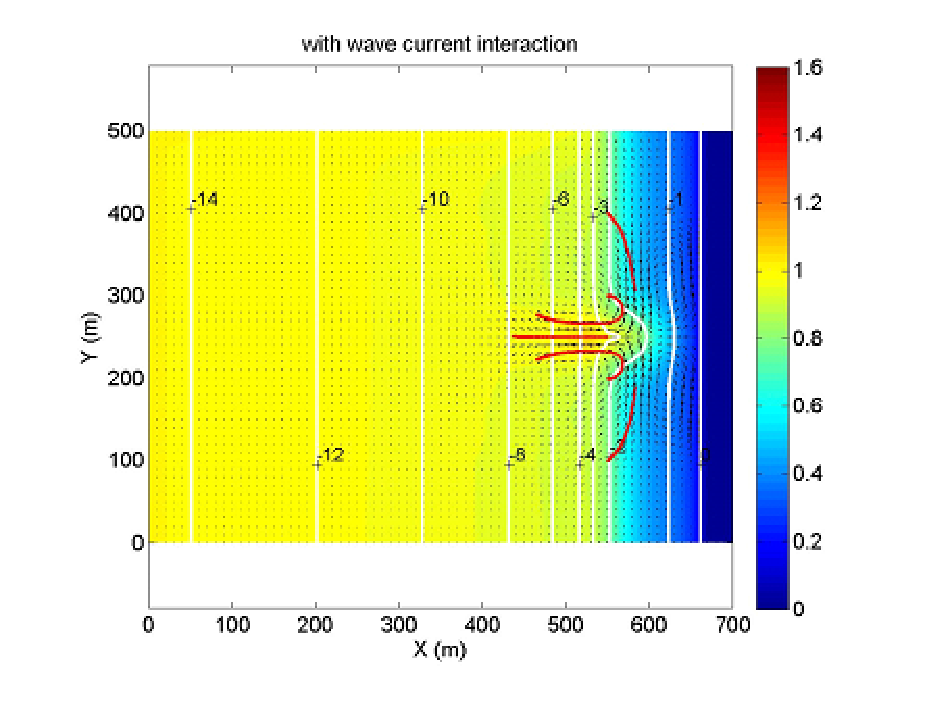
\includegraphics[width=0.6\textwidth]{image21}
  \caption{Example of drifter path output}
  \label{fig:image21}
\end{figure}

\section{ Discharge boundaries (river input) (advanced option)}

It is possible to define river discharges to simulate the inflow from a river (i.e. uni-directional, no tides) and no sediment transport. 

The user can define a number of sections along the boundaries of the grid through which discharges can be defined as time series. For each boundary section, the program checks how many grid cell centers lie within the section, given in world coordinates. The total length of the section is computed as the sum of the lengths of the grid cells along the boundary, and each cell length divided by this total length is used to divide the discharge over the cells within the boundary section.  

For each boundary section a separate time series of total discharge is defined; actual discharges are determined by interpolation in time. Positive discharges mean discharges into the model.

The discharges may be defined on initially dry boundaries. They must, however be located on otherwise closed (``wall'') boundaries, see parameter (``back''\_

The discharge boundaries are activated with the following keywords in \textit{params.txt}:

disch\_loc\_file=$<$\textit{discharge locations file}$>$

disch\_timeseries\_file=$<$\textit{discharge timeseries file$>$}

The contents of the discharge locations file are a number of records equal to the number of discharge boundary sections, with for each record four numbers:

\textit{X\_begin Y\_begin X\_end Y\_end}

\textit{}

These world coordinates must be chosen such that they are close to the desired boundary and enclose the cell centers of the cells that must be part of the boundary section.

In the discharge time series file, the first column is time in seconds; the next columns give the total discharge time series per section.

\textit{Example: (River Outflow)}

disch\_loc\_file=discharge\_locations.txt

disch\_timeseries\_file=discharge\_timeseries.txt

\textit{Contents of discharge\_locations.txt:}

840 820 840 890

\textit{Contents of discharge\_timeseries.txt:}

0 150

1000000 150

\textbf{}

\begin{figure}[h]
  \centering
  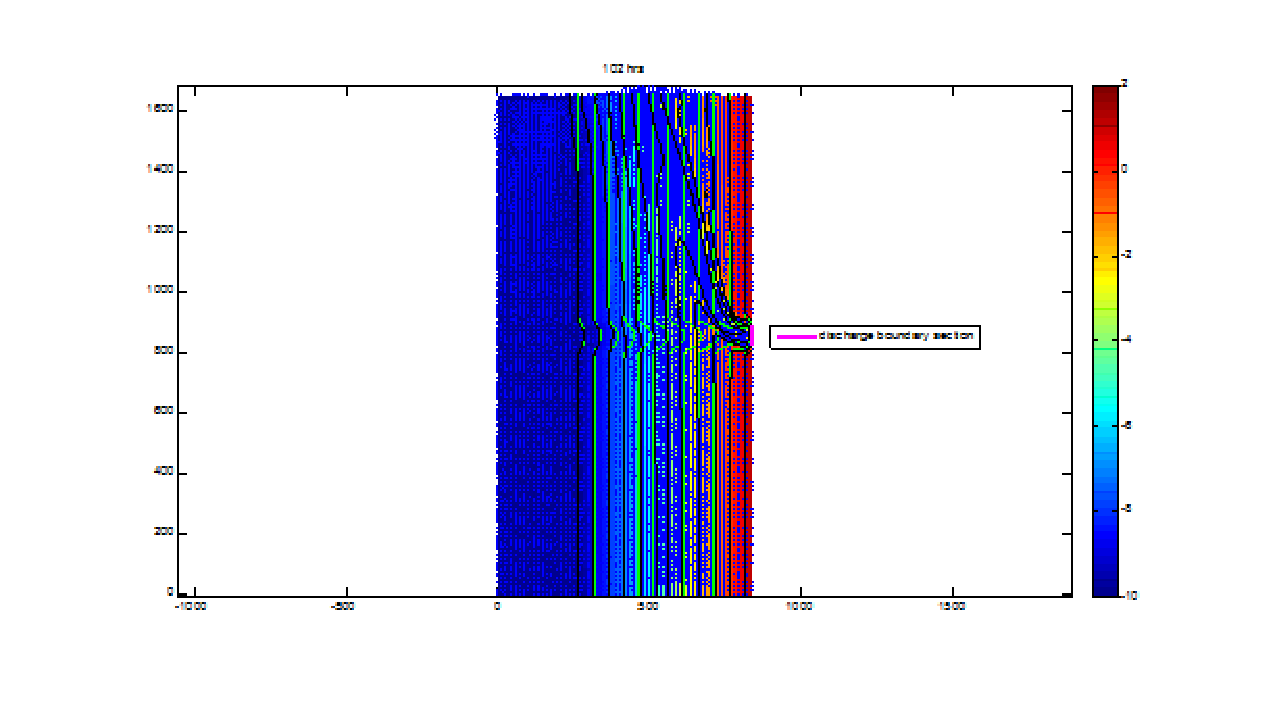
\includegraphics[width=0.6\textwidth]{image22}
  \caption{Example of coast with river inflow}
  \label{fig:image22}
\end{figure}

\section{ Dam break (advanced option)}

Dam break problems require the same set of hydrodynamic equations which XBeach contains. The only difference between these types of problems and convential coastal model is the specification of the innitial condition file for the water level.

An non-uniform initial condition for the water level, for instance when modeling a dam break problem, can be specified by a file with the same format as the depth file. It is activated by the following keyword in \textit{params.txt}:

\textit{zsinitfile = $<$initial condition file$>$}

\textit{Example (Dambreak)}

Zsinitfile=ini.dep

\begin{figure}[h]
  \centering
  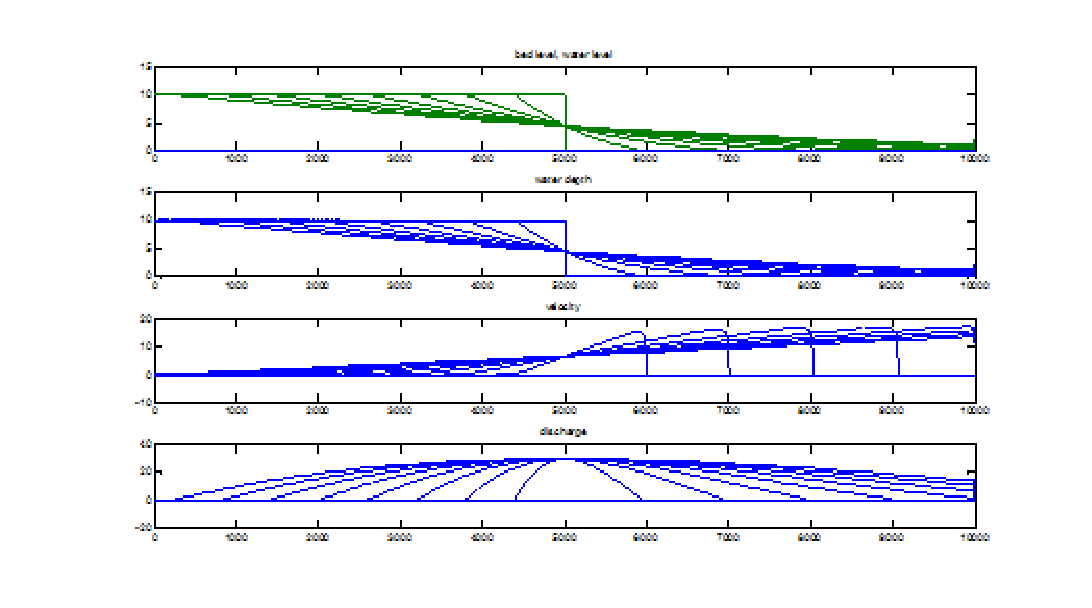
\includegraphics[width=0.6\textwidth]{image23}
  \caption{Dam break problem: snapshots of the water level, water depth, velocity and discharge}
  \label{fig:image23}
\end{figure}

%%% Local Variables: 
%%% mode: latex
%%% TeX-master: "xbeach_manual"
%%% End: 
